% =====================================================================
%  FoodYou -- Nominal-Behaviour Conformance Campaign
%  Result report for the fault-free ("happy") test purpose.
%  Overleaf-ready, self-contained: pdflatex twice.
% =====================================================================
\documentclass[11pt,a4paper]{article}

\usepackage[utf8]{inputenc}
\usepackage[T1]{fontenc}
\usepackage[margin=2.4cm]{geometry}
\usepackage{booktabs}
\usepackage{multirow}
\usepackage{array}
\usepackage{xcolor}
\usepackage{listings}
\usepackage{amssymb}
\usepackage{caption}
\usepackage{tikz}
\usetikzlibrary{arrows.meta,positioning,fit,shapes.geometric,calc,backgrounds}
\usepackage[hidelinks]{hyperref}

\definecolor{codebg}{gray}{0.96}
\definecolor{accent}{RGB}{0,90,160}
\definecolor{warn}{RGB}{176,60,20}
\definecolor{good}{RGB}{20,110,60}

\lstset{
  basicstyle=\ttfamily\footnotesize,
  backgroundcolor=\color{codebg},
  frame=single, rulecolor=\color{gray!40},
  breaklines=true, columns=fullflexible,
  xleftmargin=0pt, framexleftmargin=4pt, aboveskip=8pt, belowskip=6pt
}

\newcommand{\gate}[1]{\texttt{\small #1}}
\newcommand{\dref}[1]{\textbf{D#1}}

\title{\vspace{-1.5em}\textbf{FoodYou: Nominal-Behaviour Conformance Campaign}\\[0.3em]
\large Result report for the fault-free test purpose, prior to disruption testing}
\author{}
\date{Campaign closed 19 August 2026}

\begin{document}
\maketitle
\vspace{-2.5em}

\begin{center}
\begin{minipage}{0.93\textwidth}
\small\itshape
All figures are measured from the artefacts listed in Section~\ref{sec:repro}.
Figures that are inferred rather than measured are labelled as such at the point
of use. Runs predating the framework corrections of 17--19 August 2026
(Section~\ref{sec:defects}) are not comparable and are not quoted.
\end{minipage}
\end{center}

\vspace{0.8em}

% =====================================================================
\section{Objective}
% =====================================================================

The disruption results this project exists to produce are meaningful only if a
\textsc{fail} on the fault-free path means what it says. This campaign establishes
that baseline and asks two questions:

\begin{description}
  \item[RQ1] Does FoodYou conform to its nominal specification under \textbf{ioco}?
  \item[RQ2] Are the verdicts \emph{sound} --- is every reported \textsc{fail} one
        the tester actually earned?
\end{description}

\noindent\textbf{RQ1: yes.} 102 generated test cases, \textbf{zero conformance
counter-examples}, across 503 observed \gate{CONFIRM\_TOTAL} outputs and 558
independent arithmetic checks.

\noindent\textbf{RQ2: not initially.} Every \textsc{fail} observed during the
campaign traced to a defect in the \emph{test framework}, not the SUT. Four
distinct defects were found and corrected. This is reported as a primary result
(Section~\ref{sec:defects}), because an ioco concretization layer is itself a
program that can be wrong --- and being wrong in the direction of a false
\textsc{fail} is indistinguishable from a discovery unless it is actively hunted.

% =====================================================================
\section{Campaign timeline and what changed}
% =====================================================================

The result in Section~\ref{sec:results} is not the output of a single run. It is
the output of the framework as it stood on 19 August 2026, after the corrections
in Table~\ref{tab:timeline}. The table is included because the trajectory is part
of the finding: the same suite shape produced 54 failures before these changes and
zero after.

\begin{table}[h]
\centering
\caption{Changes made during the campaign, and why.}
\label{tab:timeline}
\footnotesize
\begin{tabular}{@{}p{1.9cm} p{5.1cm} p{8.4cm}@{}}
\toprule
\textbf{Date} & \textbf{Change} & \textbf{Reason} \\
\midrule
13 Aug & \gate{el\_search\_results} selector tightened; \texttt{external\_dependencies}
guard \emph{retired} &
The selector had matched the query echoed in the search box, so a zero-result
search satisfied its own precondition. The guard was retired on the belief that the
external branch would now stop at that precondition --- a belief later shown false
(\dref{4}). \\
\addlinespace
17 Aug & \dref{1}, \dref{2}, \dref{3} corrected; exact-sum ledger made
fail-closed; findings surfaced independently of verdicts; evidence captured on
oracle rejection &
The tester was selecting among the SUT's outputs, and the oracle was unreachable
from one of two execution paths. See Section~\ref{sec:defects}. \\
\addlinespace
18 Aug & Full 102-case sweep executed; \dref{4} diagnosed; missing
\gate{wait\_for (el\_search\_results)} added to the external arm of the System
Interface &
All 13 failures had one cause. The System Interface fix is composed into the test
cases at generation time and is therefore \emph{inert until regeneration}. \\
\addlinespace
19 Aug & \texttt{external\_dependencies} guard reinstated;
external coverage gap measured against the catalogue API &
Restores the correct verdict without a CADP cycle, using framework support that had
been deliberately left in place. \\
\bottomrule
\end{tabular}
\end{table}

% =====================================================================
\section{Subject under test}
% =====================================================================

\begin{table}[h]
\centering\footnotesize
\caption{Subject.}
\begin{tabular}{@{}ll@{}}
\toprule
Application & FoodYou (\texttt{com.maksimowiczm.foodyou}) \\
Domain & Local-first calorie and nutrition tracker \\
Platform & Android; Kotlin, Jetpack Compose \\
Persistence & Room / SQLite (\texttt{open\_source\_database.db}) \\
Catalogues & Swiss Food Composition Database (bundled, offline); Open Food Facts
(remote); user-defined; recent history \\
Driver & Appium, UiAutomator2 automation backend \\
UI identification & No resource-ids (Compose): text and content-description
selectors only \\
\bottomrule
\end{tabular}
\end{table}

FoodYou snapshots nutrition values into the diary entry at log time
(\texttt{DiaryProduct}); a logged entry does not track later catalogue changes.
This constrains what a staleness disruption can mean and is recorded here for the
campaign that follows.

% =====================================================================
\section{Model, generation and concretization}
% =====================================================================

\begin{figure}[h]
\centering
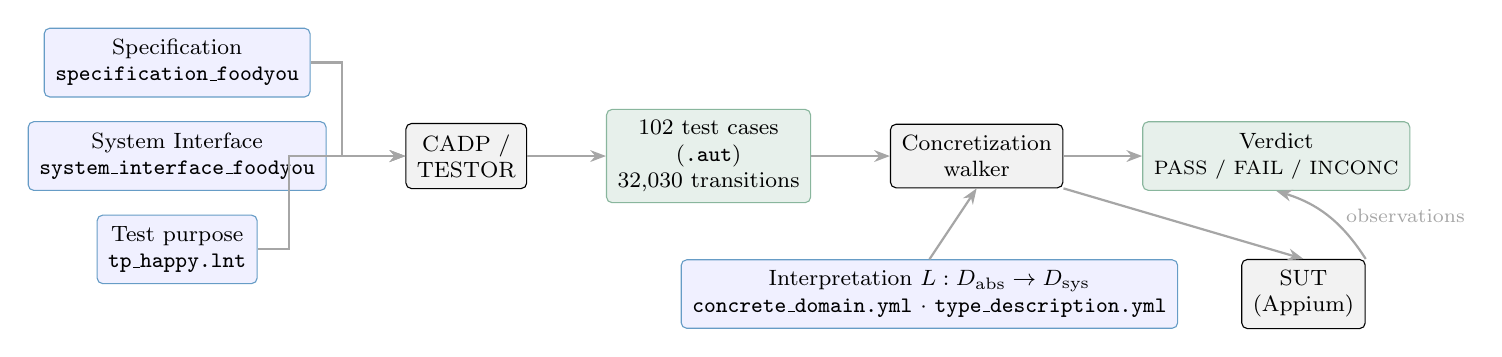
\begin{tikzpicture}[
  font=\footnotesize,
  box/.style={draw, rounded corners=2pt, minimum height=8mm, align=center, inner sep=4pt},
  model/.style={box, fill=blue!6, draw=accent!60},
  tool/.style={box, fill=gray!10},
  art/.style={box, fill=good!10, draw=good!50},
  ar/.style={-{Stealth[length=2mm]}, thick, gray!70}
]
\node[model] (spec) {Specification\\\texttt{specification\_foodyou}};
\node[model, below=3mm of spec] (si) {System Interface\\\texttt{system\_interface\_foodyou}};
\node[model, below=3mm of si] (tp) {Test purpose\\\texttt{tp\_happy.lnt}};

\node[tool, right=10mm of si] (testor) {CADP /\\TESTOR};
\node[art, right=10mm of testor] (auts) {102 test cases\\(\texttt{.aut})\\32{,}030 transitions};
\node[tool, right=10mm of auts] (walk) {Concretization\\walker};
\node[art, right=10mm of walk] (verd) {Verdict\\{\scriptsize PASS / FAIL / INCONC}};

\node[model, below=9mm of walk, xshift=-6mm] (interp)
  {Interpretation $L : D_{\mathrm{abs}} \rightarrow D_{\mathrm{sys}}$\\
   \texttt{concrete\_domain.yml} $\cdot$ \texttt{type\_description.yml}};
\node[tool, right=8mm of interp] (sut) {SUT\\(Appium)};

\draw[ar] (spec.east) -- ++(4mm,0) |- (testor.west);
\draw[ar] (si.east) -- (testor.west);
\draw[ar] (tp.east) -- ++(4mm,0) |- (testor.west);
\draw[ar] (testor) -- (auts);
\draw[ar] (auts) -- (walk);
\draw[ar] (walk) -- (verd);
\draw[ar] (interp.north) -- (walk.south);
\draw[ar] (walk.south east) -- (sut.north);
\draw[ar] (sut.north east) to[bend right=20] node[right,pos=0.5,xshift=1mm]{\scriptsize observations} (verd.south);
\end{tikzpicture}
\caption{Generation and concretization pipeline. The System Interface is
\emph{composed into} the test cases, so its concrete steps are fixed at generation
time --- the fact underlying \dref{4}'s remediation cost.}
\label{fig:pipeline}
\end{figure}

\subsection{Suite shape}

\begin{table}[h]
\centering\footnotesize
\caption{Generated suite (102 controllable test cases).}
\label{tab:suite}
\begin{tabular}{@{}lrrr@{}}
\toprule
& \textbf{min} & \textbf{median} & \textbf{max} \\
\midrule
States per test case & 58 & 216 & 255 \\
Transitions per test case & 88 & 323 & 381 \\
\midrule
\multicolumn{4}{@{}l@{}}{Total transitions across the suite: \textbf{32{,}030}} \\
\multicolumn{4}{@{}l@{}}{Gates in the System Interface: \textbf{17}} \\
\bottomrule
\end{tabular}
\end{table}

Test cases are \emph{controllable}: at most one input is enabled per state. This is
what makes the tester's behaviour determined by the test case rather than by its
own choices --- the property \dref{1} and \dref{2} violated in practice.

\subsection{Abstract domain and fixture}

\gate{DailyTotal} is a \emph{saturating band}, not an exact figure:
\{\textsc{empty}, \textsc{low}, \textsc{moderate}, \textsc{high}, \textsc{over}\}.
The specification counts committed entries --- one rung per entry --- and the
concretization inverts this as
$\mathrm{rung} = \mathrm{round}(\mathrm{observed\ kcal} / \mathrm{bucket\ unit})$.

\medskip
\noindent\fbox{\begin{minipage}{0.96\textwidth}\small
\textbf{Stated validity condition (from the model itself).} The band inversion is
valid \emph{only while every logged entry is the same food}. This is not concealed;
it is the reason the exact-sum oracle exists.
\end{minipage}}
\medskip

\begin{table}[h]
\centering\footnotesize
\caption{Fixture. Energies are read back from the application's own \texttt{Product}
table, never asserted by the harness.}
\label{tab:fixture}
\begin{tabular}{@{}lllr@{}}
\toprule
\textbf{Abstract} & \textbf{Product} & \textbf{Catalogue} & \textbf{kcal / 100\,g} \\
\midrule
\texttt{food\_peanut} & Peanut butter & Swiss FCD & 636 \\
\texttt{food\_butter} & Cooking butter & Swiss FCD & 745 \\
\texttt{food\_oil} & Corn germ oil & Swiss FCD & 900 \quad(\texttt{defaultF}) \\
\bottomrule
\end{tabular}
\end{table}

Daily goal 2000\,kcal; band rungs 0 / 900 / 1800 / 2700 / 3600. The three energies
are deliberately spread so that a total composed of different foods cannot be
mistaken for a whole number of portions. \texttt{seed\_foods.sh} verifies these
values before every run and aborts if they do not hold, so a drifted fixture fails
loudly rather than producing quietly wrong verdicts.

% =====================================================================
\section{Timing constants}
% =====================================================================

All waits are bounded and declared; none is implicit in the test logic.

\begin{table}[h]
\centering\footnotesize
\caption{Timing constants in force during the campaign.}
\label{tab:timing}
\begin{tabular}{@{}llp{7.8cm}@{}}
\toprule
\textbf{Constant} & \textbf{Value} & \textbf{Role} \\
\midrule
\texttt{-{}-timeout} & 10\,s & Observation and precondition budget for every
\texttt{wait\_for} and \texttt{observe}. Overridable per sweep via
\texttt{TIMEOUT}; 10\,s used throughout this campaign. \\
\texttt{wait\_timeout} & 10\,s & The same budget, plumbed into the executor
adapter and the Android executor so no wait silently uses a different one. \\
Appium implicit wait & 2\,s & Per-\texttt{find} budget inside a single wait. \\
\texttt{newCommandTimeout} & 300\,s & Session keep-alive; not a test parameter. \\
Settle delay (post-navigation) & 0.6\,s & Allows the next screen to compose before
the following find. \\
Settle delay (pre-typing) & 0.5\,s & Allows the view to settle before text entry. \\
Settle delay (post-scroll / re-find) & 0.4\,s & Allows layout to settle after a
scroll gesture. \\
\midrule
Observed case duration & 22--133\,s & Median 55\,s ($n=102$). \\
Suite duration & $\approx$1\,h\,45\,m & 102 cases, one repetition, one emulator. \\
\bottomrule
\end{tabular}
\end{table}

\noindent\textbf{Was 10\,s adequate?} Yes, and this is checkable rather than
assumed. A wait that expires where the specification required an output is
classified \textsc{quiescence} and flagged for review; \textbf{no run in this
campaign produced a \textsc{quiescence} classification}. Every non-\textsc{pass}
outcome was a precondition failure, which is a different thing: the tester never
reached the screen where an output was owed.

% =====================================================================
\section{Oracles}
% =====================================================================

Four checks run per observation, layered so the weakest is never the only one
active. This layering is what makes ``zero counter-examples'' a claim rather than
an absence of evidence.

\begin{table}[h]
\centering\footnotesize
\caption{Oracle inventory.}
\label{tab:oracles}
\begin{tabular}{@{}lp{6.4cm}p{5.4cm}@{}}
\toprule
\textbf{Oracle} & \textbf{Compares} & \textbf{Sensitivity} \\
\midrule
Band & Observed total mapped to an abstract bucket, against the bucket the test
case expects & Coarse: tolerates $\pm\tfrac{1}{2}$ portion ($\pm$450\,kcal at a
900\,kcal portion) \\
\addlinespace
Exact-sum & Displayed total against the running sum of what the tester actually
logged & Exact, to the calorie; valid on mixed-food diaries \\
\addlinespace
Arithmetic & Whether the total is a whole number of portions & Fallback when
energies are undeclared \\
\addlinespace
Delta & Whether the total moved by the amount the last diary action implies &
Fallback; single-food only \\
\addlinespace
\gate{FOOD\_INFO} & Displayed per-food energy against the application's own
catalogue value & Exact \\
\bottomrule
\end{tabular}
\end{table}

\subsection{Findings are not verdicts}

An exact-sum mismatch is reported as a \emph{finding}, not a verdict: the
specification states bands, so an exact discrepancy violates nothing it asserts.
Findings therefore never terminate a walk --- which means they can ride inside a
\textsc{pass}. They are consequently counted and reported separately in the sweep
output, and a \textsc{pass} is not treated as self-certifying.

\subsection{The ledger fails closed}

The exact-sum oracle maintains a running sum. \gate{ADD\_ENTRY} and
\gate{REMOVE\_ENTRY} cannot check anything themselves --- no total is on screen at
that point --- so each \emph{stages} its movement for the next
\gate{CONFIRM\_TOTAL} to apply. One slot, one producer, one consumer.

If a movement is already staged when the next arrives, the consumer that should
have applied it was never reached. The ledger then declares itself \textsc{unknown}
and \textbf{abstains for the remainder of the run} rather than reporting against a
sum it knows to be stale.

\medskip
\noindent\fbox{\begin{minipage}{0.96\textwidth}\small
\textbf{Design rationale.} An oracle that abstains costs one missed check. An
oracle that is quietly wrong costs the credibility of every verdict in the
campaign, because nothing downstream can distinguish a manufactured
counter-example from a real one. The abstention is itself reported, so a run whose
strongest oracle switched off is visibly weaker evidence than one where it ran.
\end{minipage}}

% =====================================================================
\section{Verdict semantics: earning a \textsc{fail}}
% =====================================================================

\begin{figure}[h]
\centering
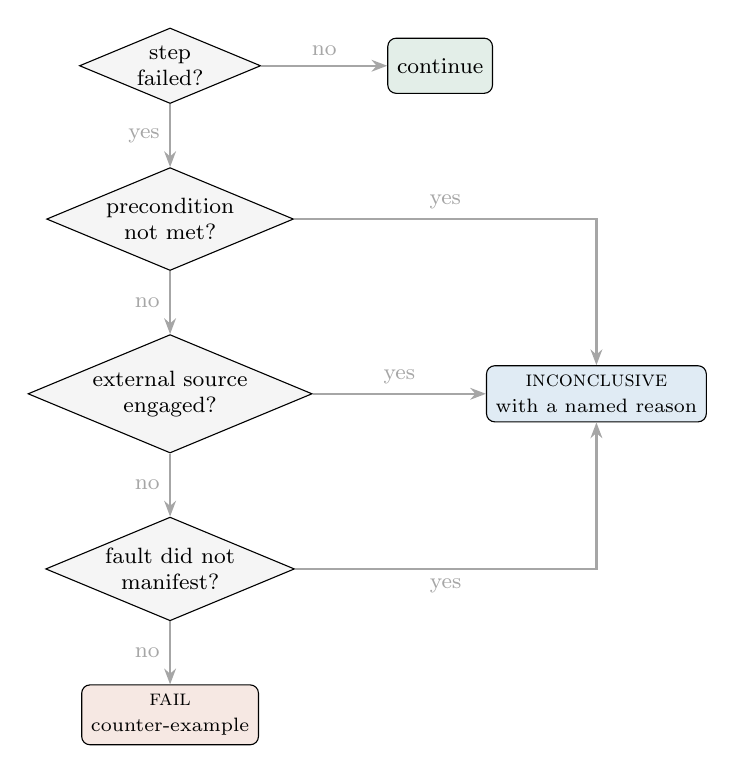
\begin{tikzpicture}[
  font=\footnotesize, node distance=6mm,
  dec/.style={draw, diamond, aspect=2.4, inner sep=1pt, align=center, fill=gray!8},
  end/.style={draw, rounded corners=3pt, minimum height=7mm, align=center},
  ar/.style={-{Stealth[length=2mm]}, thick, gray!70}
]
\node[dec] (d1) {step\\failed?};
\node[end, fill=good!12, right=16mm of d1] (pass) {continue};
\node[dec, below=8mm of d1] (d2) {precondition\\not met?};
\node[dec, below=8mm of d2] (d3) {external source\\engaged?};
\node[dec, below=8mm of d3] (d4) {fault did not\\manifest?};
\node[end, fill=warn!12, below=8mm of d4] (fail) {\textsc{fail}\\{\scriptsize counter-example}};
\node[end, fill=accent!12, right=22mm of d3] (inc) {\textsc{inconclusive}\\{\scriptsize with a named reason}};

\draw[ar] (d1) -- node[above]{no} (pass);
\draw[ar] (d1) -- node[left]{yes} (d2);
\draw[ar] (d2) -- node[left]{no} (d3);
\draw[ar] (d3) -- node[left]{no} (d4);
\draw[ar] (d4) -- node[left]{no} (fail);
\draw[ar] (d2.east) -| node[pos=0.25,above]{yes} (inc.north);
\draw[ar] (d3.east) -- node[above]{yes} (inc.west);
\draw[ar] (d4.east) -| node[pos=0.25,below]{yes} (inc.south);
\end{tikzpicture}
\caption{The verdict procedure. \textsc{fail} is the \emph{last} branch, not the
default: a stimulus the tester could not apply yields no observation, so there is
nothing for the oracle to judge. All three \textsc{inconclusive} reasons resolve
through a single function, so the verdict and the reported reason cannot disagree.}
\label{fig:verdict}
\end{figure}

\begin{table}[h]
\centering\footnotesize
\caption{\textsc{inconclusive} reasons, in evaluation order.}
\label{tab:inconc}
\begin{tabular}{@{}rp{5.2cm}p{7.6cm}@{}}
\toprule
& \textbf{Reason} & \textbf{Meaning} \\
\midrule
1 & Executor precondition failure & A \texttt{wait\_for}-only selector never
appeared: the gate's screen was not up, so the tester was not in control. Distinct
from an \emph{oracle} selector, which also appears in an \texttt{observe} block and
whose absence \emph{is} evidence about the SUT. \\
\addlinespace
2 & External data source engaged and the fixture cannot populate it & The walk
selected a catalogue outside the SUT that the fixture cannot fill; everything
downstream fails for want of data. \textbf{All 13 non-\textsc{pass} cases in this
campaign.} \\
\addlinespace
3 & Fault target did not manifest & An injection was a no-op, so no disruption was
actually applied. Not exercised in this fault-free campaign. \\
\bottomrule
\end{tabular}
\end{table}

\noindent The precondition/oracle distinction in reason~1 is derived
mechanically from the System Interface: a selector appearing in an
\texttt{observe} block is an oracle selector, everything else in a
\texttt{wait\_for} is a precondition. \dref{4} was a failure of exactly this
distinction.

% =====================================================================
\section{Results}
\label{sec:results}
% =====================================================================

\begin{table}[h]
\centering\footnotesize
\caption{Verdict distribution, 102 test cases.}
\label{tab:verdicts}
\begin{tabular}{@{}lrl@{}}
\toprule
\textbf{Verdict} & \textbf{Count} & \textbf{Status} \\
\midrule
\textsc{pass} & 89 / 102 & measured \\
\textsc{inconclusive} & 13 / 102 & \textbf{3 measured, 10 inferred}
(Section~\ref{sec:threats}) \\
\textsc{fail} (conformance counter-example) & \textbf{0} & measured \\
\bottomrule
\end{tabular}
\end{table}

\noindent\textbf{No test case produced a conformance counter-example.} Every
non-\textsc{pass} verdict is a case in which the tester could not apply its
stimulus and therefore obtained no observation to judge.

\begin{table}[h]
\centering\footnotesize
\caption{Oracle activity across the 102-case sweep.}
\label{tab:activity}
\begin{tabular}{@{}lr@{}}
\toprule
\gate{CONFIRM\_TOTAL} band checks & 558 \\
Exact-sum ledger applications & 558 \\
\gate{FOOD\_INFO} authoritative-value checks & 165 \\
\midrule
Arithmetic / delta / exact-sum \textbf{findings} & \textbf{0} \\
Ledger abstentions & \textbf{0} \\
\textsc{quiescence} classifications & \textbf{0} \\
\bottomrule
\end{tabular}
\end{table}

Every observed \gate{CONFIRM\_TOTAL} reached both the band and the exact-sum
oracle; the two never disagreed with the device, and the ledger never lost track.

\begin{table}[h]
\centering\footnotesize
\caption{Gate coverage. Note that \gate{VIEW\_DIARY}, \gate{DIARY\_INFO} and
\gate{REMOVE\_ENTRY} do \emph{not} appear in the body of \texttt{tp\_happy.lnt}.}
\label{tab:coverage}
\begin{tabular}{@{}lrr@{}}
\toprule
\textbf{Gate} & \textbf{Cases reaching it} & \textbf{Total firings} \\
\midrule
\gate{SEARCH\_FOOD} & 102 & 178 \\
\gate{FOOD\_INFO} & 98 & 165 \\
\gate{ADD\_ENTRY} & 97 & 471 \\
\gate{CONFIRM\_TOTAL} & 97 & 503 \\
\gate{REMOVE\_ENTRY} & 72 & 87 \\
\gate{VIEW\_DIARY} & 6 & 6 \\
\gate{DIARY\_INFO} & 6 & 6 \\
\bottomrule
\end{tabular}
\end{table}

\noindent A TESTOR test purpose is a \emph{selector over the composed
specification}, not a script: gates absent from the purpose body are still woven
into the generated cases. \gate{REMOVE\_ENTRY} is exercised in every generated case
and fires 87 times, including the add--remove--add sequences that returned the
total exactly to its prior value ($3600 \rightarrow 2700 \rightarrow 3600$),
verified to the calorie.

% =====================================================================
\section{Primary finding: four defects, all in the tester}
\label{sec:defects}
% =====================================================================

No defect was found in the SUT. Four were found in the concretization framework,
each of which had been producing or concealing incorrect verdicts.

\subsection*{\dref{1} --- The tester chose among the SUT's outputs}

A checkpoint shortcut selected among multiple abstract \emph{outputs} by
shortest-distance-to-\textsc{pass}, then failed the run when the SUT produced the
other equally-permitted one. The specification allows either
(\texttt{alt total := HIGH [] total := OVER}); which occurs is the SUT's decision,
never the tester's. \textbf{Affected 100 of 102 test cases.}

\subsection*{\dref{2} --- Branch selection ignored the observation}

The fallback matcher compared the abstract token to the rendered value literally
(\texttt{"over" == "2700 / 2000 kcal"}), which never matches, so the first
alternative won by default. The tester was still choosing --- now silently, and
with no oracle running at all. Corrected so that the \emph{observation} selects the
branch, through the same interpretation function the oracle uses. Where no
alternative is satisfied, that --- and only that --- is the counter-example, and it
is reported naming every value the specification permitted.

\subsection*{\dref{3} --- The oracle had one call site, behind a shortcut}

\begin{figure}[h]
\centering
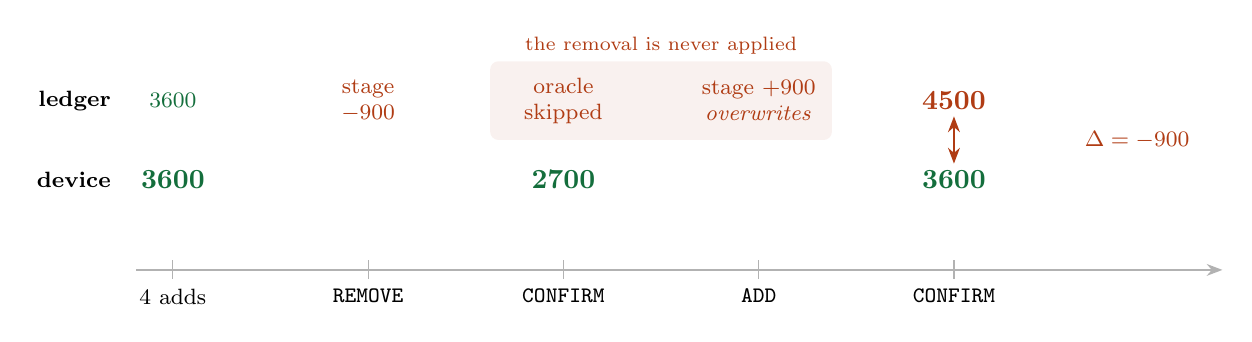
\begin{tikzpicture}[font=\footnotesize, x=1.55cm, y=1cm]
% timeline
\draw[thick,gray!60,-{Stealth[length=2mm]}] (-0.3,0) -- (8.6,0);
\foreach \x/\lab in {0/{4 adds}, 1.6/{\texttt{REMOVE}}, 3.2/{\texttt{CONFIRM}},
                     4.8/{\texttt{ADD}}, 6.4/{\texttt{CONFIRM}}}
  \draw[gray!60] (\x,0.12) -- (\x,-0.12) node[below,align=center,black]{\lab};

% device row
\node[left=2mm of {(-0.3,1.15)}, align=right] {\textbf{device}};
\foreach \x/\v in {0/3600, 1.6/{}, 3.2/2700, 4.8/{}, 6.4/3600}
  \node[good, font=\bfseries] at (\x,1.15) {\v};

% ledger row
\node[left=2mm of {(-0.3,2.15)}, align=right] {\textbf{ledger}};
\node[good] at (0,2.15) {3600};
\node[warn, align=center] at (1.6,2.15) {stage\\$-900$};
\node[warn, align=center] at (3.2,2.15) {oracle\\skipped};
\node[warn, align=center] at (4.8,2.15) {stage $+900$\\\emph{overwrites}};
\node[warn, font=\bfseries] at (6.4,2.15) {4500};

\node[warn] at (7.9,1.65) {$\Delta = -900$};
\draw[warn,thick,{Stealth[length=2mm]}-{Stealth[length=2mm]}] (6.4,1.95) -- (6.4,1.35);

\begin{scope}[on background layer]
  \fill[warn!7, rounded corners=3pt] (2.6,1.65) rectangle (5.4,2.65);
\end{scope}
\node[warn, font=\scriptsize] at (4.0,2.85) {the removal is never applied};
\end{tikzpicture}
\caption{\dref{3}: ledger desynchronisation. The device is correct at every step
($3600-900+900 = 3600$). The tester reports a confident \texttt{TOTAL MISMATCH} of
$-900$\,kcal against a total the application computed correctly.}
\label{fig:d3}
\end{figure}

\noindent The oracle entry point was reachable only from the path taken when a
state offers a single abstract transition. Every gate reached at a state offering
\emph{several} permitted outputs skipped the oracle \emph{and} the exact-sum ledger
update entirely.

\medskip
\noindent\fbox{\begin{minipage}{0.96\textwidth}\small
\textbf{The coupling that made this systematic.} The only multi-output state in the
specification is \texttt{drop(OVER)}, and the only way to reach it is a
\gate{REMOVE\_ENTRY} from \textsc{over}. So the single skipped consumer and the
single \emph{subtracting} ledger operation are the same event. Every removal from a
saturated total was guaranteed to corrupt the ledger --- not a corner case, a
structural coupling between the specification's shape and the walker's control
flow.
\end{minipage}}

\subsection*{\dref{4} --- An asymmetric System Interface turned an honest empty
result into a \textsc{fail}}

Of 14 source-selection sites in the System Interface, exactly one --- the external
catalogue branch --- omitted \gate{wait\_for (el\_search\_results)}. It proceeded
directly to \gate{wait\_for (el\_calories)}, a selector that also appears in an
\texttt{observe} block and is therefore an \emph{oracle} selector, so its timeout
was reported as a conformance failure. The application had behaved correctly: it
displayed an honest source count of 0 and ``No food found''.

\textbf{This single omission accounted for all 13 failures in the sweep.}

\medskip
\noindent\textbf{Remediation cost.} The System Interface is composed into the test
cases at generation time (Figure~\ref{fig:pipeline}), so the corrected
\texttt{wait\_for} is inert until the suite is regenerated. In the interim, the
configured external-dependency guard restores the correct verdict --- at the price
recorded in Section~\ref{sec:threats}.

\subsection{Trajectory}

An earlier campaign on a 93-case suite reported 54 failures; the 102-case suite
reports zero. These are different suites generated from different model revisions.
This is a \textbf{trajectory, not a controlled comparison}, and must not be quoted
as a measured improvement factor.

% =====================================================================
\section{Methodological measures}
% =====================================================================

Four properties were established to keep verdicts auditable. Each is stated
SUT-independently, as a requirement on any ioco concretization layer.

\begin{enumerate}\setlength\itemsep{2pt}
  \item \textbf{The observation selects the branch.} Where a specification permits
  several outputs, the tester reads the value and follows the branch the
  observation satisfies. Choosing among outputs is not the tester's right.
  \item \textbf{The oracle runs on every accepted transition}, not only on those
  reached by a structural shortcut.
  \item \textbf{Cross-step bookkeeping fails closed.} State the oracle maintains
  across steps is invalidated the moment it can be shown to have lost an update,
  and the check abstains rather than reporting.
  \item \textbf{Findings are surfaced independently of verdicts.} Checks that
  cannot terminate a walk are counted per run, so a suite of \textsc{pass}es is a
  clean result only if the findings column is clean too.
\end{enumerate}

\noindent Additionally, evidence (screenshot and UI tree) is captured when an
\emph{oracle} rejects an observation, not only when a wait times out. The case that
most needs a picture is the one where the tester found the value and the oracle
disagreed --- precisely a candidate counter-example.

% =====================================================================
\section{Threats to validity}
\label{sec:threats}
% =====================================================================

\subsection*{Construct validity}
The \gate{DailyTotal} band inverts correctly only while every logged entry is the
same food. Mitigated by the exact-sum oracle, which is mixed-food safe and ran 558
times without disagreement --- but the band remains the abstraction the
specification is written in. \gate{WriteStatus} is internal and never directly
observed; \gate{CONFIRM\_TOTAL} is the only window onto it.

\subsection*{Internal validity}
\textbf{The framework was defective during part of the campaign.} All figures in
Section~\ref{sec:results} are post-correction; earlier runs are not comparable and
are not quoted.

\textbf{The external-dependency guard masks defects by construction.} Any failure
downstream of selecting the external catalogue is downgraded to
\textsc{inconclusive}, so a genuine SUT defect on that path would be hidden. This
is an explicit, configured trade-off and is the reason the external branch is
reported as a coverage gap rather than as a pass. It costs nothing under the
present fixture, because that branch cannot produce evidence either way
(Section~\ref{sec:gaps}).

\textbf{A single repetition.} The full sweep ran at one repetition per case.
Stability was confirmed on a subset (identical verdicts on repeat), but a
suite-wide flakiness rate has not been measured. This is the weakest point in the
present evidence.

\subsection*{Reliability of the \textsc{inconclusive} figure}
Of the 13 \textsc{inconclusive} cases, \textbf{3 were re-run and confirmed}
(variants 12, 30, 91) after the guard was reinstated. The remaining 10 share an
identical cause, gate and selector but \textbf{have not been individually re-run}.
The figure is therefore 3 measured and 10 inferred, and should be completed before
publication.

\subsection*{External validity}
One application, one test purpose, one device, one Android image. No claim of
generality across applications or platforms is made from this campaign alone.

% =====================================================================
\section{What is \emph{not} claimed --- coverage gaps}
\label{sec:gaps}
% =====================================================================

\begin{table}[h]
\centering\footnotesize
\caption{Untested surfaces, stated explicitly.}
\begin{tabular}{@{}p{4.2cm}p{11.2cm}@{}}
\toprule
\textbf{Gap} & \textbf{Detail} \\
\midrule
External catalogue branch never exercised &
All 13 \textsc{inconclusive} cases query Open Food Facts for
\texttt{defaultF} = Corn germ oil, which returns \textbf{0 results} --- confirmed
twice independently: by the application's own displayed source count, and by direct
query to the catalogue API. This is \textbf{not} a limitation of the catalogue: the
same API returns \textbf{215 results} for ``Cooking butter''. Every System Interface
branch fixes \texttt{fid := defaultF}, so the external source is only ever queried
for the one product it does not carry. \emph{A fixture choice, not an environmental
constraint.} \\
\addlinespace
Quantity never varied &
Every \gate{ADD\_ENTRY} uses the application default of 100\,g, giving exactly
900\,kcal. All arithmetic checks ran on round numbers; rounding and off-by-one
behaviour in the quantity path is untested. \\
\addlinespace
Only one food ever logged &
No mixed-food diary was constructed, so the band oracle's stated validity condition
was never actually stressed on device. \\
\addlinespace
Unit conversion (g\,$\leftrightarrow$\,ml) never ran &
No unit control is declared in the interpretation layer. \\
\addlinespace
\gate{VIEW\_DIARY} / \gate{DIARY\_INFO} thinly covered &
6 firings each, against 503 for \gate{CONFIRM\_TOTAL}. \\
\bottomrule
\end{tabular}
\end{table}

% =====================================================================
\section{Reproduction}
\label{sec:repro}
% =====================================================================

\begin{lstlisting}
source EVALUATION/foodyou/env.sh        # asserts device, network, catalogue, fixture energies

bash EVALUATION/foodyou/run_variants.sh happy                       # full suite

python framework/scripts/classify_failure.py \                   # classify one run,
  EVALUATION/foodyou/generated/variant_logs/happy/v<N>.log           # incl. hidden findings

REPEATS=3 bash EVALUATION/foodyou/investigate_variants.sh happy <N>...  # repeat + diagnostics
\end{lstlisting}

\noindent\texttt{env.sh} refuses to proceed on a device that cannot reach the
network, or whose fixture foods do not hold their authoritative energies, so a
poisoned environment fails loudly rather than producing a sweep of quiet false
results.

\medskip
\noindent\textbf{Artefacts.}
\texttt{EVALUATION/foodyou/variants\_happy.log} (suite verdicts);
\texttt{generated/variant\_logs/happy/} (per-case stdout+stderr);
\texttt{generated/investigate/happy/} (repeat runs);
\texttt{tmp/failure\_artifacts/} (screenshots and UI trees captured at the moment of
rejection).

% =====================================================================
\section{Before the disruption campaign}
% =====================================================================

Ordered by effect on the credibility of the disruption results.

\begin{enumerate}\setlength\itemsep{2pt}
  \item \textbf{Re-run the remaining 10 \textsc{inconclusive} cases} so
  Table~\ref{tab:verdicts} is fully measured.
  \item \textbf{Measure suite-wide flakiness} --- at minimum a stratified
  three-repetition subset. Currently the weakest point in the evidence.
  \item \textbf{Regenerate the test cases}, folding in the \dref{4} System
  Interface correction; then reconsider whether the guard --- which masks defects
  by construction --- can be withdrawn.
  \item \textbf{Point the external branch at a product the catalogue carries}, with
  the authoritative energy resolved \emph{per source}. Converts 13
  \textsc{inconclusive}s into 13 real verdicts.
  \item \textbf{Vary quantity} over a small bounded set (e.g.\ 100 / 137 / 250\,g).
  Requires quantity to become a gate parameter, the declared energy to become a
  function of quantity, and the exact-sum ledger to scale accordingly. The largest
  untested surface, and the one the strongest oracle is built for.
  \item \textbf{Converge the oracle's two call sites onto one.} Disruption branches
  will add further multi-output states --- the shape that produced \dref{3}.
\end{enumerate}

\noindent Items 4 and 5 share a CADP cycle and should be done together. Bound the
quantity domain to a few values rather than a range: an earlier extraction reached
323 variants before being cancelled, and generation cost will otherwise dominate.

\end{document}
